%
%   Copyright 2013 Katarzyna Szawan <kat.szwn@gmail.com>
%       and Michał Rus <m@michalrus.com>
%
%   Licensed under the Apache License, Version 2.0 (the "License");
%   you may not use this file except in compliance with the License.
%   You may obtain a copy of the License at
%
%       http://www.apache.org/licenses/LICENSE-2.0
%
%   Unless required by applicable law or agreed to in writing, software
%   distributed under the License is distributed on an "AS IS" BASIS,
%   WITHOUT WARRANTIES OR CONDITIONS OF ANY KIND, either express or implied.
%   See the License for the specific language governing permissions and
%   limitations under the License.
%

\documentclass{beamer}
\usepackage[utf8]{inputenc}
\usepackage[T1]{fontenc}
\usepackage[english]{babel}
\usepackage{graphicx}
\usepackage{times}

\usepackage{xkeyval}
\usepackage{todonotes}
\presetkeys{todonotes}{inline}{}

\usetheme{AGH}

\title[Mindmapping system]{Mindmapping system for Android}

\author[Szawan, Rus, Wojnicki]{Katarzyna Szawan\\Michał Rus\\dr inż. Igor Wojnicki}

\date[2014]{2014/01/28}

\institute[AGH-UST]
{Wydział EAIiB\\ 
Katedra Informatyki Stosowanej
}

\setbeamertemplate{itemize item}{$\maltese$}

\begin{document}

{
%\usebackgroundtemplate{
\includegraphics[width=\paperwidth]{titlepage}} % wersja angielska
\usebackgroundtemplate{
\includegraphics[width=\paperwidth]{titlepagepl}} % wersja polska
 \begin{frame}
   \titlepage
 \end{frame}
}

%---------------------------------------------------------------------------

\begin{frame}
\frametitle{Mapy myśli}

	\todo[inline]{To było niewidoczne z naszej pozycji, a co dopiero z publiczności.}

	\begin{figure}
		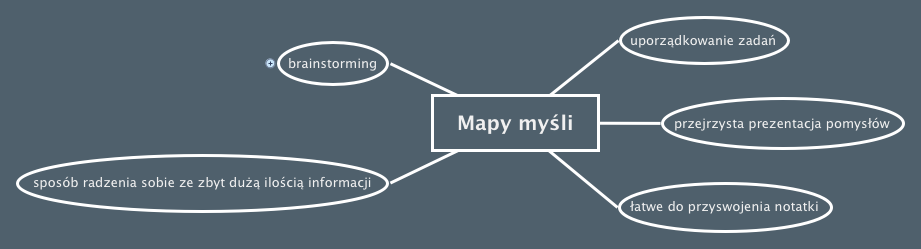
\includegraphics[width=\textwidth]{mind-map}
	\end{figure}

\end{frame}

\begin{frame}
\frametitle{Nasze rozwiązanie --- dla end-usera}

\todo{Że na Androida.}

\todo{Że import.}

\todo{Figura z wycinkiem z XMinda! Zrobi wrażenie?}

\todo{Że synchronizacja online i offline.}

\todo{Że banalne w obsłudze --- genialny UX!}

\end{frame}
\begin{frame}
\frametitle{Android + Akka + Spray.io}

\begin{columns}[c]
	\begin{column}[t]{.45\textwidth}
		\vskip-5em
		\begin{enumerate}
			\item Scala na Androidzie --- można?
			\only<2->{\item Serwer(y): Akka + Spray.io.
				\item Telefon --- aktor.}
			\only<3->{\item Push? REST Spray.io z long-pollingiem.
				\item To samo API dla webapp.}
		\end{enumerate}
	\end{column}
	\begin{column}{.45\textwidth}
		\begin{figure}
			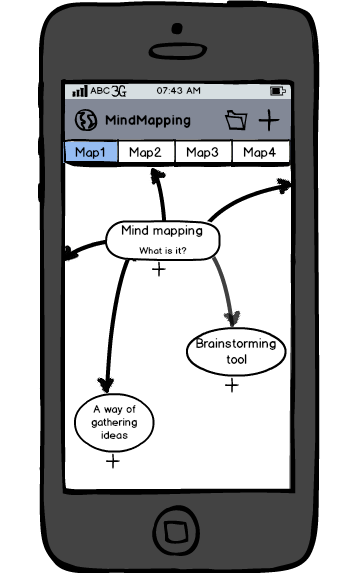
\includegraphics[height=6cm]{graphics-mockup-map}
		\end{figure}
	\end{column}
\end{columns}

\end{frame}

%
%   Copyright 2013 Katarzyna Szawan <kat.szwn@gmail.com>
%       and Michał Rus <m@michalrus.com>
%
%   Licensed under the Apache License, Version 2.0 (the "License");
%   you may not use this file except in compliance with the License.
%   You may obtain a copy of the License at
%
%       http://www.apache.org/licenses/LICENSE-2.0
%
%   Unless required by applicable law or agreed to in writing, software
%   distributed under the License is distributed on an "AS IS" BASIS,
%   WITHOUT WARRANTIES OR CONDITIONS OF ANY KIND, either express or implied.
%   See the License for the specific language governing permissions and
%   limitations under the License.
%

\begin{frame}[t]
\frametitle{Kolaboracja on-line}

\vskip+6em

\begin{itemize}
	\item Synchronizacja \emph{stosunkowo} prosta --- dane: drzewo.
	\item Określone z góry chunki --- node'y drzewa.
\end{itemize}

\only<2->{\begin{center}
	\Large Node = (time, UUID, content, parent Node)
\end{center}}

\only<3->{\begin{itemize}
  \item Tylko czas serwera/-ów!
\end{itemize}}

\end{frame}

\begin{frame}
\frametitle{Synchronizacja off-line}

\todo{O automatycznym rozwiązywaniu konfliktów.}
\todo{Dwa typy konfliktu: content i placement.}
\todo{O prezentowaniu konfliktów end-userowi.}

\end{frame}
\begin{frame}
\frametitle{Subtree recreation algorithm --- kiedy?}

\begin{columns}[c]
	\begin{column}[t]{.45\textwidth}
		\vskip-4em
		\begin{enumerate}
			\item Wspólny stan.
			\only<2,3,4>{\item Usunięcie poddrzewa on-line.}
			\only<3,4>{\item Dodanie node'a off-line.}
			\only<4>{\item Odtworzenie poddrzewa.}
		\end{enumerate}
	\end{column}
	\begin{column}{.45\textwidth}
		\begin{figure}
			\includegraphics<1>[height=6cm]{recreation-1}
			\includegraphics<2>[height=6cm]{recreation-2}
			\includegraphics<3>[height=6cm]{recreation-3}
			\includegraphics<4>[height=6cm]{recreation-4}
		\end{figure}
	\end{column}
\end{columns}

\end{frame}

%
%   Copyright 2013 Katarzyna Szawan <kat.szwn@gmail.com>
%       and Michał Rus <m@michalrus.com>
%
%   Licensed under the Apache License, Version 2.0 (the "License");
%   you may not use this file except in compliance with the License.
%   You may obtain a copy of the License at
%
%       http://www.apache.org/licenses/LICENSE-2.0
%
%   Unless required by applicable law or agreed to in writing, software
%   distributed under the License is distributed on an "AS IS" BASIS,
%   WITHOUT WARRANTIES OR CONDITIONS OF ANY KIND, either express or implied.
%   See the License for the specific language governing permissions and
%   limitations under the License.
%

\chapter{Summary}
\label{chap:summary}

\section{Testing the applications}
\label{summary-testing}
\todo[inline,caption={Conducted tests}]{\michal{K., shall we involve some random people in using our app and\ldots observe them? \kasia{I'd put here short information about manual tests, the impression of users and some backend performance  statistics maybe?}} \michal{Sounds great!}}

\todo[inline,caption={How the reqs were met: implications, consequences, values(?)}]{\\\michal{K., well, isn't this already present in \cref{summary-how-solve}?}}

\section{How does the implementation solve the problem?}
\label{summary-how-solve}
\todo[inline]{How does the implementation solve the problem?}
\todo[inline]{Remind about the objective.}
The aims of our work are put in \cref{sec:requirements}. Now we will sum up what we managed to implement. 
 
The first objective was to create an application compatible with XMind which lets its users create, edit and display mind maps. We succeeded in this task: our application enables creating, editing, displaying and deleting mind maps.

Next, there was a part about presenting maps in a clean, structured way. We believe our application meets tis requirement. We put a lot of effort in positioning mind nodes, bidirectional scroll view also turned out to be troublesome and it is described in the \cref{sec:impl-problems}.

\section{What is missing in our solution?}
\label{summary-missing}
\todo[inline]{Were all problems solved? If not: why?}
The Android application is visually compatibile with XMind only on a very basic level. The main reason for that is that that was not the main issue while creating the software. We wanted to focus on creating the \emph{collaboration} tool. Still, a better compatibility would definitely be beneficial. 

When it comes to the UI, we did not implement subtree folding, which seems a basic functionality in mind mapping software (althought not mentioned in our requirements). Also, the feature of moving any node (reassigning its parent node) by long-pressing it and choosing `Change parent' option, and then tapping on the new parent-to-be was not implemented. At that point, there was not enough time left to add it.

\section{Future works}
\label{summary-future}
When it comes to what could be done next, some of the things we would like to see implemented include:

\begin{itemize}
	\item adding users, privileges, explicit sharing etc. (the most important feature the system is now lacking),
	\item better XMind compatibility, support for node--node relations, folding, floating objects and attachments, custom icons, as well as some predefined styles,
	\item a web application using only static HTML/JS/CSS files (and, what's most important, \emph{the same} highly-scalable Akka as a backend),
	\item a move of Akka's storage from PostgreSQL to a more scalable NoSQL store (probably MongoDB),
	\item an involvement of a professional UI designer; having him draw all UI elements would add to a beautiful user experience,
	\item making use of a new \inlinecode{akka-cluster} Akka subproject to have no central/main Akka node; instead, a completely self-organizing cluster of servers would be more fault-tolerant,
	\item adding map-wide blocking of currently-edited node for other, non-editing users to improve the UX even more.
\end{itemize}


%---------------------------------------------------------------------------

\end{document}
